% Options for packages loaded elsewhere
\PassOptionsToPackage{unicode}{hyperref}
\PassOptionsToPackage{hyphens}{url}
\PassOptionsToPackage{dvipsnames,svgnames,x11names}{xcolor}
%
\documentclass[
  letterpaper,
  DIV=11,
  numbers=noendperiod]{scrartcl}

\usepackage{amsmath,amssymb}
\usepackage{iftex}
\ifPDFTeX
  \usepackage[T1]{fontenc}
  \usepackage[utf8]{inputenc}
  \usepackage{textcomp} % provide euro and other symbols
\else % if luatex or xetex
  \usepackage{unicode-math}
  \defaultfontfeatures{Scale=MatchLowercase}
  \defaultfontfeatures[\rmfamily]{Ligatures=TeX,Scale=1}
\fi
\usepackage{lmodern}
\ifPDFTeX\else  
    % xetex/luatex font selection
\fi
% Use upquote if available, for straight quotes in verbatim environments
\IfFileExists{upquote.sty}{\usepackage{upquote}}{}
\IfFileExists{microtype.sty}{% use microtype if available
  \usepackage[]{microtype}
  \UseMicrotypeSet[protrusion]{basicmath} % disable protrusion for tt fonts
}{}
\makeatletter
\@ifundefined{KOMAClassName}{% if non-KOMA class
  \IfFileExists{parskip.sty}{%
    \usepackage{parskip}
  }{% else
    \setlength{\parindent}{0pt}
    \setlength{\parskip}{6pt plus 2pt minus 1pt}}
}{% if KOMA class
  \KOMAoptions{parskip=half}}
\makeatother
\usepackage{xcolor}
\setlength{\emergencystretch}{3em} % prevent overfull lines
\setcounter{secnumdepth}{-\maxdimen} % remove section numbering
% Make \paragraph and \subparagraph free-standing
\ifx\paragraph\undefined\else
  \let\oldparagraph\paragraph
  \renewcommand{\paragraph}[1]{\oldparagraph{#1}\mbox{}}
\fi
\ifx\subparagraph\undefined\else
  \let\oldsubparagraph\subparagraph
  \renewcommand{\subparagraph}[1]{\oldsubparagraph{#1}\mbox{}}
\fi


\providecommand{\tightlist}{%
  \setlength{\itemsep}{0pt}\setlength{\parskip}{0pt}}\usepackage{longtable,booktabs,array}
\usepackage{calc} % for calculating minipage widths
% Correct order of tables after \paragraph or \subparagraph
\usepackage{etoolbox}
\makeatletter
\patchcmd\longtable{\par}{\if@noskipsec\mbox{}\fi\par}{}{}
\makeatother
% Allow footnotes in longtable head/foot
\IfFileExists{footnotehyper.sty}{\usepackage{footnotehyper}}{\usepackage{footnote}}
\makesavenoteenv{longtable}
\usepackage{graphicx}
\makeatletter
\def\maxwidth{\ifdim\Gin@nat@width>\linewidth\linewidth\else\Gin@nat@width\fi}
\def\maxheight{\ifdim\Gin@nat@height>\textheight\textheight\else\Gin@nat@height\fi}
\makeatother
% Scale images if necessary, so that they will not overflow the page
% margins by default, and it is still possible to overwrite the defaults
% using explicit options in \includegraphics[width, height, ...]{}
\setkeys{Gin}{width=\maxwidth,height=\maxheight,keepaspectratio}
% Set default figure placement to htbp
\makeatletter
\def\fps@figure{htbp}
\makeatother

\usepackage{booktabs}
\usepackage{longtable}
\usepackage{array}
\usepackage{multirow}
\usepackage{wrapfig}
\usepackage{float}
\usepackage{colortbl}
\usepackage{pdflscape}
\usepackage{tabu}
\usepackage{threeparttable}
\usepackage{threeparttablex}
\usepackage[normalem]{ulem}
\usepackage{makecell}
\usepackage{xcolor}
\KOMAoption{captions}{tableheading}
\makeatletter
\makeatother
\makeatletter
\makeatother
\makeatletter
\@ifpackageloaded{caption}{}{\usepackage{caption}}
\AtBeginDocument{%
\ifdefined\contentsname
  \renewcommand*\contentsname{Table of contents}
\else
  \newcommand\contentsname{Table of contents}
\fi
\ifdefined\listfigurename
  \renewcommand*\listfigurename{List of Figures}
\else
  \newcommand\listfigurename{List of Figures}
\fi
\ifdefined\listtablename
  \renewcommand*\listtablename{List of Tables}
\else
  \newcommand\listtablename{List of Tables}
\fi
\ifdefined\figurename
  \renewcommand*\figurename{Figure}
\else
  \newcommand\figurename{Figure}
\fi
\ifdefined\tablename
  \renewcommand*\tablename{Table}
\else
  \newcommand\tablename{Table}
\fi
}
\@ifpackageloaded{float}{}{\usepackage{float}}
\floatstyle{ruled}
\@ifundefined{c@chapter}{\newfloat{codelisting}{h}{lop}}{\newfloat{codelisting}{h}{lop}[chapter]}
\floatname{codelisting}{Listing}
\newcommand*\listoflistings{\listof{codelisting}{List of Listings}}
\makeatother
\makeatletter
\@ifpackageloaded{caption}{}{\usepackage{caption}}
\@ifpackageloaded{subcaption}{}{\usepackage{subcaption}}
\makeatother
\makeatletter
\@ifpackageloaded{tcolorbox}{}{\usepackage[skins,breakable]{tcolorbox}}
\makeatother
\makeatletter
\@ifundefined{shadecolor}{\definecolor{shadecolor}{rgb}{.97, .97, .97}}
\makeatother
\makeatletter
\makeatother
\makeatletter
\makeatother
\ifLuaTeX
  \usepackage{selnolig}  % disable illegal ligatures
\fi
\IfFileExists{bookmark.sty}{\usepackage{bookmark}}{\usepackage{hyperref}}
\IfFileExists{xurl.sty}{\usepackage{xurl}}{} % add URL line breaks if available
\urlstyle{same} % disable monospaced font for URLs
\hypersetup{
  pdftitle={Hypothesis Testing},
  pdfauthor={Mallory Barnes},
  colorlinks=true,
  linkcolor={blue},
  filecolor={Maroon},
  citecolor={Blue},
  urlcolor={Blue},
  pdfcreator={LaTeX via pandoc}}

\title{Hypothesis Testing}
\author{Mallory Barnes}
\date{}

\begin{document}
\maketitle
\ifdefined\Shaded\renewenvironment{Shaded}{\begin{tcolorbox}[frame hidden, breakable, interior hidden, boxrule=0pt, borderline west={3pt}{0pt}{shadecolor}, sharp corners, enhanced]}{\end{tcolorbox}}\fi

\begin{center}\rule{0.5\linewidth}{0.5pt}\end{center}

\hypertarget{hypothesis-testing}{%
\section{Hypothesis Testing}\label{hypothesis-testing}}

Hypothesis testing is a way to decide if a certain statement about a
population might be true based on sample data.

\begin{center}\rule{0.5\linewidth}{0.5pt}\end{center}

\hypertarget{clarifying-alpha-p-value-and-confidence-level}{%
\subsection{Clarifying Alpha, P-value, and Confidence
Level}\label{clarifying-alpha-p-value-and-confidence-level}}

\hypertarget{alpha-alpha}{%
\paragraph{\texorpdfstring{Alpha
(\(\alpha\))}{Alpha (\textbackslash alpha)}}\label{alpha-alpha}}

Alpha (\(\alpha\)) is the significance level of a statistical test, and
it quantifies the risk of committing a Type I error. A Type I error
happens when we incorrectly reject a true null hypothesis. The standard
value for alpha is often set at 0.05, implying a 5\% chance of making a
Type I error. In other words, we are willing to accept a 5\% risk of
concluding that a difference exists when there is no actual difference.

\hypertarget{p-value}{%
\paragraph{P-value}\label{p-value}}

The p-value is another crucial concept in hypothesis testing. It
represents the probability of observing the obtained results, or
something more extreme, assuming that the null hypothesis is true. A
small p-value (usually ≤ 0.05) suggests that the observed data is
inconsistent with the null hypothesis, and thus, you have evidence to
reject it.

\hypertarget{confidence-level}{%
\paragraph{Confidence Level}\label{confidence-level}}

The confidence level is related but distinct from alpha and p-value.
While alpha quantifies the risk of a Type I error, the confidence level
indicates how confident we are in our statistical estimates. The
confidence level is calculated as the complement of alpha:

Confidence Level = 1 - \(\alpha\)

For example, if α is 0.05, the confidence level would be (1 - 0.05 =
0.95) or 95\%. This means we are 95\% confident that our results fall
within a specific range.

\hypertarget{bringing-it-all-together}{%
\paragraph{Bringing It All Together}\label{bringing-it-all-together}}

\begin{itemize}
\tightlist
\item
  \textbf{Alpha (\(\alpha\))}: Risk of Type I error (usually 5\%)
\item
  \textbf{P-value}: Probability of observed data given the null is true
\item
  \textbf{Confidence Level}: Confidence in the range of our estimates
  (usually 95\%)
\end{itemize}

Understanding the relationship and differences between these three
concepts is crucial for accurate and meaningful interpretation of
statistical tests.

\begin{center}\rule{0.5\linewidth}{0.5pt}\end{center}

\hypertarget{example}{%
\subsection{Example:}\label{example}}

Let's say we want to know if the average pollution in a set of water
samples is above the legal limit. Or if young deer in a region are, on
average, healthy.

\hypertarget{step-1-define-your-hypotheses}{%
\paragraph{Step 1: Define Your
Hypotheses}\label{step-1-define-your-hypotheses}}

First, we need to define two hypotheses: the \textbf{research
hypothesis} and the \textbf{null hypothesis}.

\begin{itemize}
\tightlist
\item
  \textbf{Research Hypothesis (H\textsubscript{a})}: This is what we aim
  to support. \textbf{Remember, we can never ``prove''
  H\textsubscript{a}, only fail to reject H\textsubscript{0}}. It can
  take a few forms based on the question:

  \begin{itemize}
  \tightlist
  \item
    H\textsubscript{a}: average pollution \textgreater{} legal limit
    (pollution is too high)
  \item
    H\textsubscript{a}: average pollution \textless{} legal limit
    (pollution is too low)
  \item
    H\textsubscript{a}: average pollution ≠ legal limit (pollution is
    just different)
  \end{itemize}
\item
  \textbf{Null Hypothesis (H\textsubscript{0})}: This is the default or
  `no change' scenario. It's opposite to the research hypothesis.

  \begin{itemize}
  \tightlist
  \item
    H\textsubscript{0}: average pollution ≤ legal limit (for the first
    H\textsubscript{a})
  \item
    H\textsubscript{0}: average pollution ≥ legal limit (for the second
    H\textsubscript{a})
  \item
    H\textsubscript{0}: average pollution = legal limit (for the third
    H\textsubscript{a})
  \end{itemize}
\end{itemize}

\hypertarget{step-2-choose-your-test-statistic}{%
\paragraph{Step 2: Choose Your Test
Statistic}\label{step-2-choose-your-test-statistic}}

Based on the data, we'll compute a \textbf{test statistic}. This number
will help us decide which hypothesis seems more likely.

\hypertarget{step-3-determine-the-rejection-region}{%
\paragraph{Step 3: Determine the Rejection
Region}\label{step-3-determine-the-rejection-region}}

Before running the test, we decide on a \textbf{rejection region}. If
our test statistic falls in this region, we'll reject the null
hypothesis.

\hypertarget{step-4-check-assumptions}{%
\paragraph{Step 4: Check Assumptions}\label{step-4-check-assumptions}}

Before drawing conclusions, ensure that the test's conditions and
assumptions are satisfied.

\hypertarget{step-5-draw-conclusions}{%
\paragraph{Step 5: Draw Conclusions}\label{step-5-draw-conclusions}}

Finally, based on the test statistic and the rejection region, decide
whether to reject the null hypothesis.

\begin{center}\rule{0.5\linewidth}{0.5pt}\end{center}

\hypertarget{errors-in-hypothesis-testing}{%
\section{Errors in Hypothesis
Testing}\label{errors-in-hypothesis-testing}}

Sometimes, even with the best methods, we make incorrect decisions.

\begin{itemize}
\item
  \textbf{Type I Error (}\(\alpha\)): This happens when we mistakenly
  reject the true null hypothesis. Imagine wrongly accusing someone
  innocent. Typically, \(\alpha\) is set at 0.05 (5\%).
\item
  \textbf{Type II Error (}\(\beta\)): Here, we mistakenly accept a false
  null hypothesis. Think of it as letting a guilty person go free.
\end{itemize}

\begin{longtable}[]{@{}
  >{\raggedright\arraybackslash}p{(\columnwidth - 4\tabcolsep) * \real{0.2603}}
  >{\raggedright\arraybackslash}p{(\columnwidth - 4\tabcolsep) * \real{0.3562}}
  >{\raggedright\arraybackslash}p{(\columnwidth - 4\tabcolsep) * \real{0.3836}}@{}}
\toprule\noalign{}
\begin{minipage}[b]{\linewidth}\raggedright
Decision
\end{minipage} & \begin{minipage}[b]{\linewidth}\raggedright
If the null hypothesis is True
\end{minipage} & \begin{minipage}[b]{\linewidth}\raggedright
If the null hypothesis is False
\end{minipage} \\
\midrule\noalign{}
\endhead
\bottomrule\noalign{}
\endlastfoot
\textbf{Reject H\textsubscript{0}} & Type I error (prob = \(\alpha\)) &
Correct (prob = 1 - \(\beta\)) \\
\textbf{Fail to reject H\textsubscript{0}} & Correct (prob = 1 -
\(\alpha\)) & Type II error (prob = \(\beta\)) \\
\end{longtable}

\begin{quote}
\textbf{Key Takeaway}: As \(\alpha\) gets smaller, \(\beta\) gets
bigger, and vice-versa.
\end{quote}

\begin{center}\rule{0.5\linewidth}{0.5pt}\end{center}

\hypertarget{one-tail-or-two}{%
\section{One Tail or Two?}\label{one-tail-or-two}}

Consider our pollution scenario, where the historic pollution level was
10.0 ppb. We can set our hypotheses as:

\begin{itemize}
\item
  \textbf{H\textsubscript{0}}: pollution = 10.0 ppb. This is a
  two-tailed test. We want to know if the pollution is either
  significantly higher or lower than 10 ppb.
\item
  \textbf{H\textsubscript{0}}: pollution \textless{} 10.0 ppb. A
  one-tailed test. We're checking if pollution might be significantly
  above 10 ppb.
\item
  \textbf{H\textsubscript{0}}: pollution \textgreater{} 10.0 ppb.
  Another one-tailed test. We're seeing if pollution might be
  significantly below 10 ppb.
\end{itemize}

\begin{center}\rule{0.5\linewidth}{0.5pt}\end{center}

\hypertarget{deciphering-significance-with-p-values}{%
\section{Deciphering Significance with
P-values}\label{deciphering-significance-with-p-values}}

The p-value gives us an idea of how strange our data would appear if the
null hypothesis were indeed accurate.

\begin{itemize}
\item
  \textbf{One-Tailed Test}: The p-value shows the likelihood of
  observing an average as extreme as our sample's if the null hypothesis
  stands.
\item
  \textbf{Two-Tailed Test}: This p-value represents the odds of spotting
  an average as different from the null value as our sample's.
\end{itemize}

\begin{quote}
\textbf{Rule of Thumb}: If the p-value is less than \(\alpha\), we opt
to reject the null hypothesis.
\end{quote}

\hypertarget{graphical-review}{%
\section{Graphical Review}\label{graphical-review}}

\begin{center}\rule{0.5\linewidth}{0.5pt}\end{center}

\hypertarget{key-players-in-hypothesis-testing-visualization}{%
\subsection{Key Players in Hypothesis Testing
Visualization}\label{key-players-in-hypothesis-testing-visualization}}

We define and visualize the core components essential to understanding
the graphical representations of hypothesis testing:

\begin{enumerate}
\def\labelenumi{\arabic{enumi}.}
\item
  \textbf{Null Distribution} - The hypothesized parent distribution
  under the assumption that the null hypothesis H\textsubscript{0} is
  true.
\item
  \textbf{True Parent Distribution} - The actual distribution from which
  our sample originates.
\item
  \textbf{Inferred Parent Distribution} - The parent distribution
  inferred from our sample data. This is what we conceptualize as the
  distribution of H\textsubscript{a}.
\item
  \textbf{Sampling Distribution of the Sample Mean} - Represents the
  distribution of sample means if we were to draw multiple samples from
  the parent distribution. This is crucial for making inferences about
  the \textbf{Inferred Parent Distribution}.
\end{enumerate}

\begin{figure}

{\centering 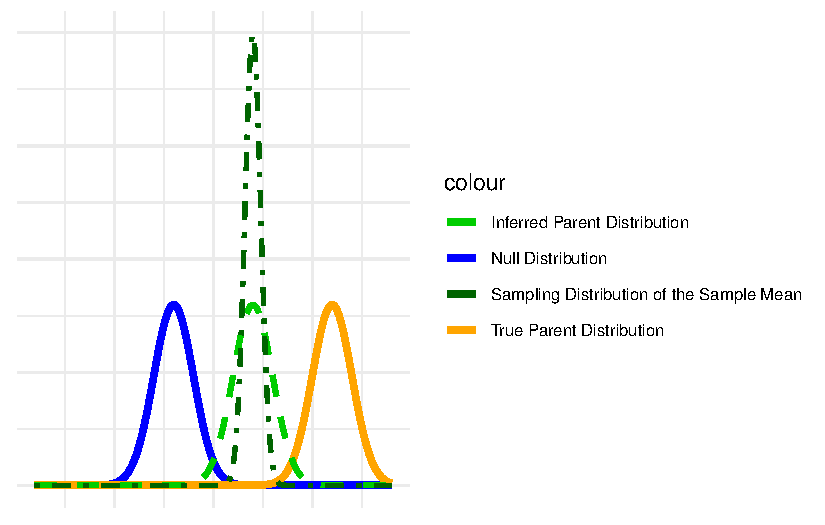
\includegraphics[width=1\textwidth,height=\textheight]{Supplemental_Chapter---Hypothesis-Testing_files/figure-pdf/fig-5-5.keyfig-1.pdf}

}

\caption{\label{fig-5-5.keyfig}This figure shows the 4 important
distributions that we need to think about with regard to hypothesis
testing.}

\end{figure}

Using the above, we can hopefully identify and understand the different
components in the hypothesis testing figures. With this in place, you
should be able to refer back to this section as a quick reference when
going through the subsequent detailed graphs.

\begin{center}\rule{0.5\linewidth}{0.5pt}\end{center}

\begin{figure}

{\centering 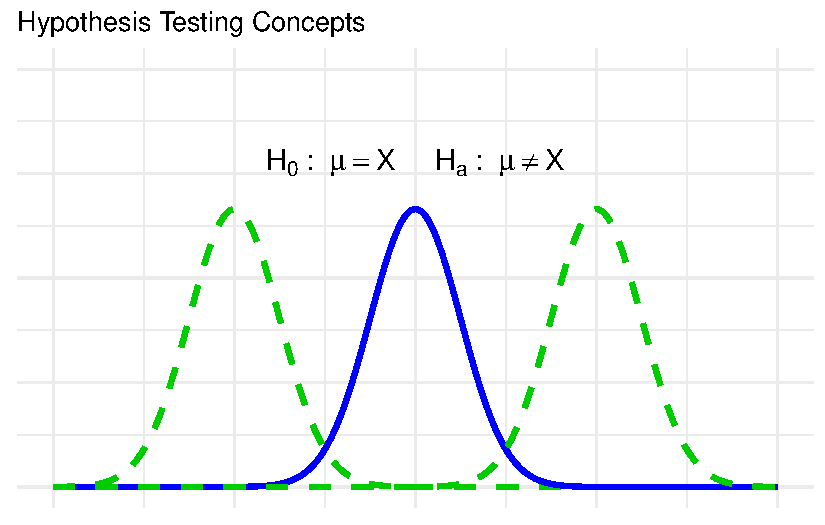
\includegraphics[width=0.75\textwidth,height=\textheight]{Supplemental_Chapter---Hypothesis-Testing_files/figure-pdf/fig-5-5.twotailed-1.pdf}

}

\caption{\label{fig-5-5.twotailed}Two-tailed distribution}

\end{figure}

For a two-tailed alternative, we are interested in the possibility that
a sample comes from a parent distribution that may have a lower or
higher location than the null.

\begin{center}\rule{0.5\linewidth}{0.5pt}\end{center}

\begin{figure}

{\centering 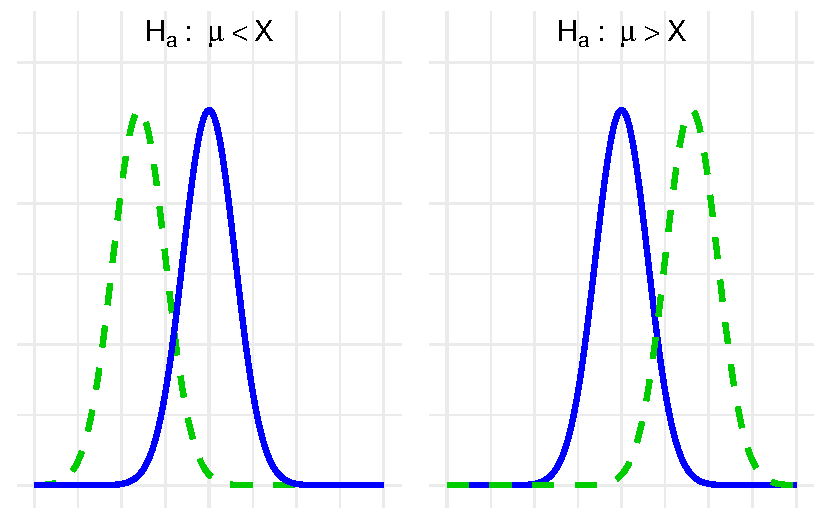
\includegraphics[width=0.75\textwidth,height=\textheight]{Supplemental_Chapter---Hypothesis-Testing_files/figure-pdf/fig-5-5.onetailed-1.pdf}

}

\caption{\label{fig-5-5.onetailed}For a one-tailed alternative, we are
interested in the possibility that a sample comes from a parent
distribution that is either at a lower or higher location than the null,
but not both.}

\end{figure}

--

\begin{figure}

{\centering 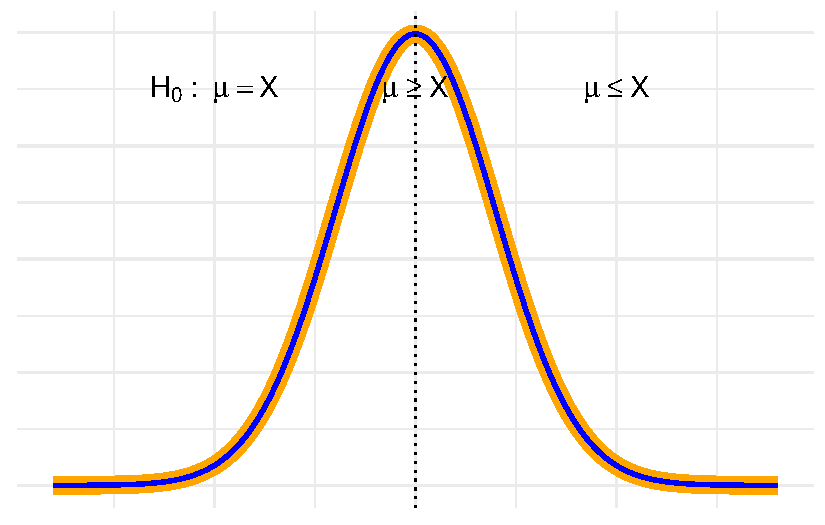
\includegraphics[width=0.75\textwidth,height=\textheight]{Supplemental_Chapter---Hypothesis-Testing_files/figure-pdf/fig-5-5.null_identical_sample-1.pdf}

}

\caption{\label{fig-5-5.null_identical_sample}\textbf{?(caption)}}

\end{figure}

In a "perfect" world in which the null hypothesis is true, the
sample\textquotesingle s parent distribution (solid, orange) is exactly
the same parent distribution described by the null hypothesis (solid,
blue).

--

\begin{figure}

{\centering 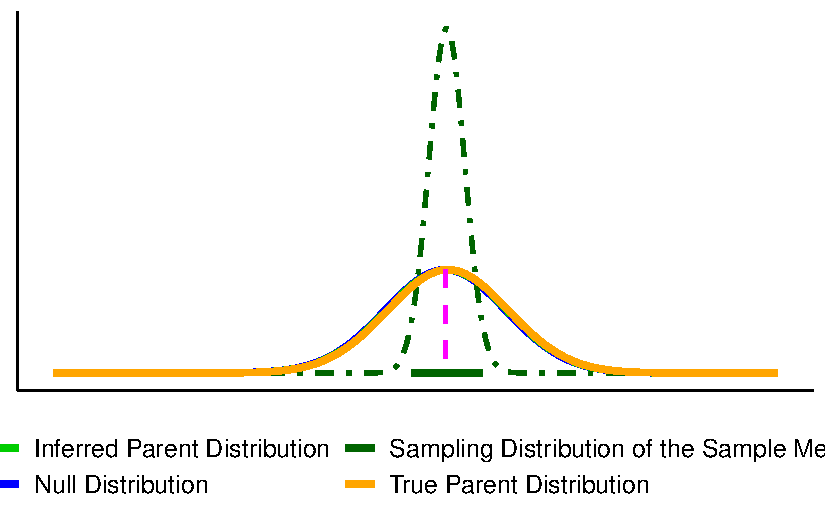
\includegraphics[width=0.75\textwidth,height=\textheight]{Supplemental_Chapter---Hypothesis-Testing_files/figure-pdf/fig-5-5.perfectly_representative_sample-1.pdf}

}

\caption{\label{fig-5-5.perfectly_representative_sample}\textbf{?(caption)}}

\end{figure}

\textbf{We never know the true parent distribution of the sample} -- we
infer it from the sample. Here, the tall dash-dotted line shows the
sampling distribution of the mean, from which we infer the parent
distribution (green3, dashed).

In this even more perfect world, that parent distribution is the same as
the parent distribution described by the null hypothesis and we have
taken a perfectly representative sample, so all 3 curves line up
perfectly on the same mean. The thick, short, flat darkgreen line is the
confidence interval for the sample mean.

\begin{center}\rule{0.5\linewidth}{0.5pt}\end{center}

\begin{figure}

{\centering 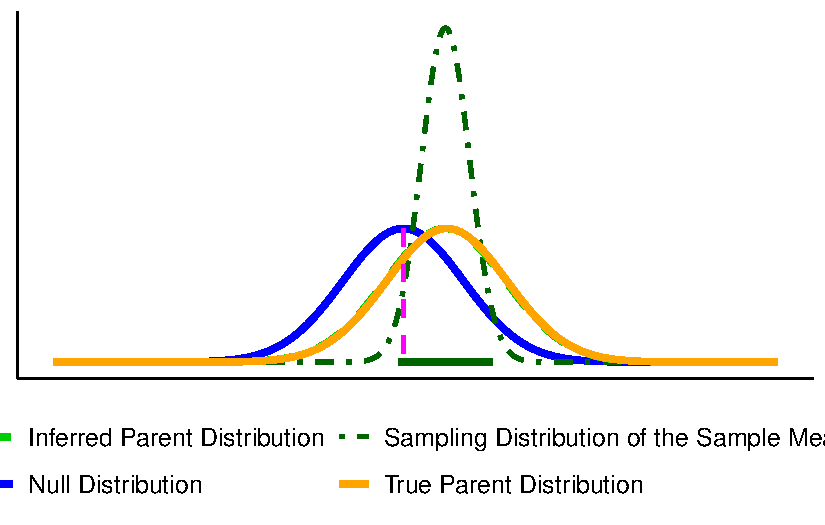
\includegraphics[width=0.75\textwidth,height=\textheight]{Supplemental_Chapter---Hypothesis-Testing_files/figure-pdf/fig-5-5.sample_imperfect_convenient-1.pdf}

}

\caption{\label{fig-5-5.sample_imperfect_convenient}\textbf{?(caption)}}

\end{figure}

In an imperfect but convenient world, the sample is not a perfect
representation of the parent population, but is fairly close. The sample
mean is close to hypothesized mean, and (in the 2-tailed case) the
confidence interval for the sample mean ``catches'' the mean of the null
hypothesis (thin solid line). A hypothesis test will correctly determine
that there is not a significant difference between the sample mean and
the mean of the null hypothesis.

\begin{center}\rule{0.5\linewidth}{0.5pt}\end{center}

\begin{figure}

{\centering 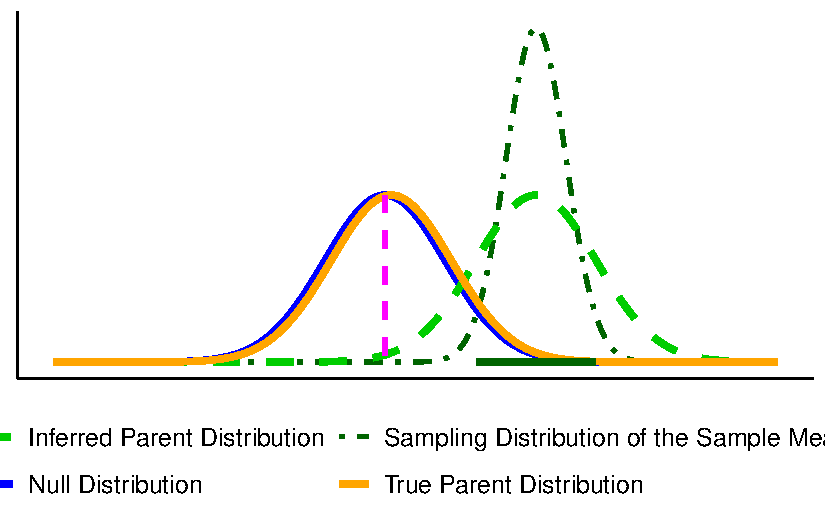
\includegraphics[width=0.75\textwidth,height=\textheight]{Supplemental_Chapter---Hypothesis-Testing_files/figure-pdf/fig-5-5.type1_error-1.pdf}

}

\caption{\label{fig-5-5.type1_error}\textbf{?(caption)}}

\end{figure}

In an imperfect and inconvenient world, the random sample is, by chance,
sufficiently imperfect that the apparent (inferred) parent distribution
is far from the true parent distribution and (in the 2-tailed case) the
confidence interval for the sample mean no longer ``catches'' the mean
of the null hypothesis. A hypothesis test will now find a significant
difference between the sample mean and the mean of the null hypothesis.
\textbf{This is a type I error}.

\begin{center}\rule{0.5\linewidth}{0.5pt}\end{center}

\begin{figure}

{\centering 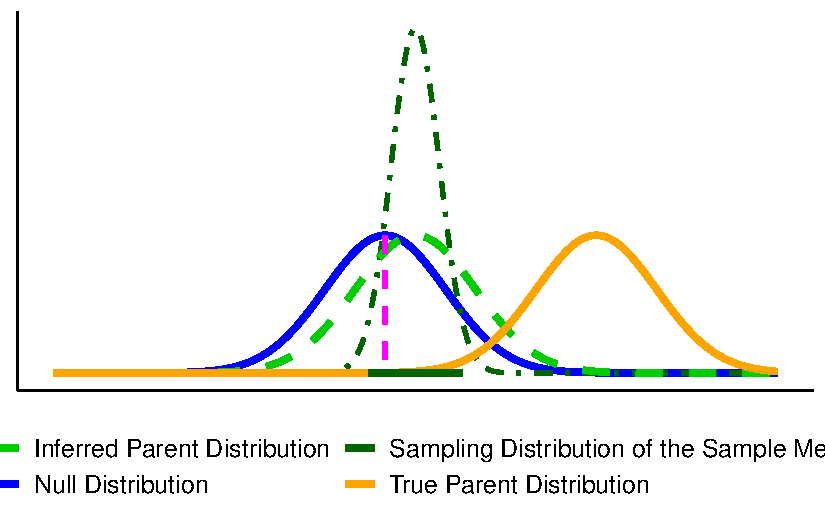
\includegraphics[width=0.75\textwidth,height=\textheight]{Supplemental_Chapter---Hypothesis-Testing_files/figure-pdf/fig-5-5.type2_error-1.pdf}

}

\caption{\label{fig-5-5.type2_error}\textbf{?(caption)}}

\end{figure}

In another imperfect and inconvenient world, the sample (dashed lines)
really is drawn from the alternative distribution (the sample's true
parent distribution; orange), but is unrepresentative of its parent and
similar to the null (solid darkgreen line). The confidence interval (in
the 2-tailed case) of the sample ``catches'' the mean of the null
hypothesis although it is far from the mean of the true parent of the
sample. A hypothesis test will find no significant difference between
the sample mean and the mean of the null hypothesis. \textbf{This is a
type II error.}

\begin{center}\rule{0.5\linewidth}{0.5pt}\end{center}

\hypertarget{graphical-review-of-test-outcomes-that-are-not-in-error}{%
\subsection{Graphical Review of Test Outcomes that are Not in
Error}\label{graphical-review-of-test-outcomes-that-are-not-in-error}}

As you review hypothesis testing, it's essential to remember that we
don't \emph{accept} the null hypothesis. The possibility of a Type I
error means our conclusion might be flawed. Instead of accepting the
null hypothesis, we \emph{fail to reject} H\textsubscript{0}. The
scarcity of data with small sample sizes can lead to significant
differences between the sample mean and the null mean (μ\_0). While it's
tempting to gather more data to be more certain, in the meantime, the
best we can do is fail to reject H\textsubscript{0}.

In the figures below, darkgreen lines represent the null parent
distribution (defined by the null mean and the sample's standard
deviation). The gray lines denote the apparent parent distribution of
our sample:

\begin{itemize}
\item
  \textbf{Solid gray line}: Represents the distribution described by our
  sample mean and standard deviation.
\item
  \textbf{Dashed gray line}: Shows the sampling distribution of the
  sample mean, described by our sample mean and the standard error (SE).
\end{itemize}

\hypertarget{graphical-descriptions}{%
\subsubsection{Graphical Descriptions:}\label{graphical-descriptions}}

\begin{enumerate}
\def\labelenumi{\arabic{enumi}.}
\item
  \textbf{Fail to Reject the Null Hypothesis - Sample Mean Supports the
  Null Hypothesis}: The means have a significant distance between them
  but not in our direction of interest. For a one-tailed test, only data
  on one side of the rejection region can support the null hypothesis.
  Question to ponder: If we gather more data and obtain the same sample
  mean, could our conclusion change?
\item
  \textbf{Fail to Reject the Null Hypothesis}: The sample mean leans
  towards the alternate hypothesis, residing on the suitable side of the
  rejection region. However, the sample size could be too small. The
  sample mean's proximity, just about 1SE from the null mean, makes it
  too close to be statistically significant. Hypothetical situation:
  With more data and the same sample mean, could our conclusion differ?
\item
  \textbf{Reject the Null Hypothesis}: The sample mean is on the right
  side of the rejection region. It's significantly distant from the null
  mean, over 3 SE, which is typically considered significant for most
  standard values of α.
\item
  \textbf{Reject the Null Hypothesis (Two-Tailed Test)}: This situation
  mirrors the previous example, but the test is two-tailed.
\end{enumerate}

\begin{center}\rule{0.5\linewidth}{0.5pt}\end{center}

\hypertarget{graphical-review-of-sample-size-effect-when-test-outcomes-are-in-error}{%
\subsection{Graphical Review of Sample Size Effect when Test Outcomes
are in
Error}\label{graphical-review-of-sample-size-effect-when-test-outcomes-are-in-error}}

It's a given that we never truly grasp the actual parent distribution of
a sample. An unrepresentative sample can lead either to a Type I or a
Type II error. The term \emph{sampling error} is sometimes invoked to
depict such unrepresentative samples, but it's imperative to understand
that the researcher hasn't committed any mistakes.

\hypertarget{graphical-descriptions-1}{%
\subsubsection{Graphical Descriptions:}\label{graphical-descriptions-1}}

\begin{enumerate}
\def\labelenumi{\arabic{enumi}.}
\setcounter{enumi}{4}
\item
  \textbf{Type I Error}: Here, the gray curve depicts both the sampling
  distribution and the apparent parent distribution of our sample. But
  in reality, the sample is a product of the null distribution. Question
  to ponder: How would the representation look if we had utilized a
  smaller sample size?
\item
  \textbf{Type II Error}: The sample genuinely hails from the solid gray
  parent population. However, it was misleading enough (as depicted by
  the dashed gray line) to seem analogous to the null distribution
  (solid darkgreen). A further rightward shift can be seen in the orange
  solid parent distribution. Query to reflect upon: How would this
  representation transform if the sample size was substantially larger?
\end{enumerate}

\begin{center}\rule{0.5\linewidth}{0.5pt}\end{center}

\hypertarget{effect-size-and-power}{%
\subsection{Effect-size and power}\label{effect-size-and-power}}

If you already know something about statistics while you were reading
this book, you might have noticed that we neglected to discuss the topic
of effect-size, and we barely talked about statistical power. We will
talk a little bit about these things here.

First, it is worth pointing out that over the years, at least in
Psychology, many societies and journals have made recommendations about
how researchers should report their statistical analyses. Among the
recommendations is that measures of ``effect size'' should be reported.
Similarly, many journals now require that researchers report an ``a
priori'' power-analysis (the recommendation is this should be done
before the data is collected). Because these recommendations are so
prevalent, it is worth discussing what these ideas refer to. At the same
time, the meaning of effect-size and power somewhat depend on your
``philosophical'' bent, and these two ideas can become completely
meaningless depending on how you think of statistics. For these
complicating reasons we have suspended our discussion of the topic until
now.

The question or practice of using measures of effect size and conducting
power-analyses are also good examples of the more general need to think
about about what you are doing. If you are going to report effect size,
and conduct power analyses, these activities should not be done blindly
because someone else recommends that you do them, these activities and
other suitable ones should be done as a part of justifying what you are
doing. It is a part of thinking about how to make your data answer
questions for you.

\hypertarget{chance-vs.-real-effects}{%
\subsubsection{Chance vs.~real effects}\label{chance-vs.-real-effects}}

Let's rehash something we've said over and over again. First,
researchers are interested in whether their manipulation causes a change
in their measurement. If it does, they can become confident that they
have uncovered a causal force (the manipulation). However, we know that
differences in the measure between experimental conditions can arise by
chance alone, just by sampling error. In fact, we can create pictures
that show us the window of chance for a given statistic, these tells us
roughly the range and likelihoods of getting various differences just by
chance. With these windows in hand, we can then determine whether the
differences we found in some data that we collected were likely or
unlikely to be due to chance. We also learned that sample-size plays a
big role in the shape of the chance window. Small samples give chance a
large opportunity make big differences. Large samples give chance a
small opportunity to make big differences. The general lesson up to this
point has been, design an experiment with a large enough sample to
detect the effect of interest. If your design isn't well formed, you
could easily be measuring noise, and your differences could be caused by
sampling error. Generally speaking, this is still a very good lesson:
better designs produce better data; and you can't fix a broken design
with statistics.

There is clearly another thing that can determine whether or not your
differences are due to chance. That is the effect itself. If the
manipulation does cause a change, then there is an effect, and that
effect is a real one. Effects refer to differences in the measurement
between experimental conditions. The thing about effects is that they
can be big or small, they have a size.

For example, you can think of a manipulation in terms of the size of its
hammer. A strong manipulation is like a jack-hammer: it is loud, it
produces a big effect, it creates huge differences. A medium
manipulation is like regular hammer: it works, you can hear it, it
drives a nail into wood, but it doesn't destroy concrete like a
jack-hammer, it produces a reliable effect. A small manipulation is like
tapping something with a pencil: it does something, you can barely hear
it, and only in a quiet room, it doesn't do a good job of driving a nail
into wood, and it does nothing to concrete, it produces tiny, unreliable
effects. Finally, a really small effect would be hammering something
with a feather, it leaves almost no mark and does nothing that is
obviously perceptiple to nails or pavement. The lesson is, if you want
to break up concrete, use a jack-hammer; or, if you want to measure your
effect, make your manipulation stronger (like a jack-hammer) so it
produces a bigger difference.

\hypertarget{effect-size-concrete-vs.-abstract-notions}{%
\subsubsection{Effect size: concrete vs.~abstract
notions}\label{effect-size-concrete-vs.-abstract-notions}}

Generally speaking, the big concept of effect size, is simply how big
the differences are, that's it. However, the biggness or smallness of
effects quickly becomes a little bit complicated. On the one hand, the
raw difference in the means can be very meaningful. Let's saw we are
measuring performance on a final exam, and we are testing whether or not
a miracle drug can make you do better on the test. Let's say taking the
drug makes you do 5\% better on the test, compared to not taking the
drug. You know what 5\% means, that's basically a whole letter grade.
Pretty good. An effect-size of 25\% would be even better right! Lot's of
measures have a concrete quality to them, and we often want to the size
of the effect expressed in terms of the original measure.

Let's talk about concrete measures some more. How about learning a
musical instrument. Let's say it takes 10,000 hours to become an expert
piano, violin, or guitar player. And, let's say you found something
online that says that using their method, you will learn the instrument
in less time than normal. That is a claim about the effect size of their
method. You would want to know how big the effect is right? For example,
the effect-size could be 10 hours. That would mean it would take you
9,980 hours to become an expert (that's a whole 10 hours less). If I
knew the effect-size was so tiny, I wouldn't bother with their new
method. But, if the effect size was say 1,000 hours, that's a pretty big
deal, that's 10\% less (still doesn't seem like much, but saving 1,000
hours seems like a lot).

Just as often as we have concrete measures that are readily
interpretable, Psychology often produces measures that are extremely
difficult to interpret. For example, questionnaire measures often have
no concrete meaning, and only an abstract statistical meaning. If you
wanted to know whether a manipulation caused people to more or less
happy, and you used to questionnaire to measure happiness, you might
find that people were 50 happy in condition 1, and 60 happy in condition
2, that's a difference of 10 happy units. But how much is 10? Is that a
big or small difference? It's not immediately obvious. What is the
solution here? A common solution is to provide a standardized measure of
the difference, like a z-score. For example, if a difference of 10
reflected a shift of one standard deviation that would be useful to
know, and that would be a sizeable shift. If the difference was only a
.1 shift in terms of standard deviation, then the difference of 10
wouldn't be very large. We elaborate on this idea next in describing
cohen's d.

\hypertarget{cohens-d}{%
\subsubsection{Cohen's d}\label{cohens-d}}

Let's look a few distributions to firm up some ideas about effect-size.
Figure~\ref{fig-5.5effectdists} has four panels. The first panel (0)
represents the null distribution of no differences. This is the idea
that your manipulation (A vs.~B) doesn't do anything at all, as a result
when you measure scores in conditions A and B, you are effectively
sampling scores from the very same overall distribution. The panel shows
the distribution as green for condition B, but the red one for condition
A is identical and drawn underneath (it's invisible). There is 0
difference between these distributions, so it represent a null effect.

\begin{figure}

{\centering 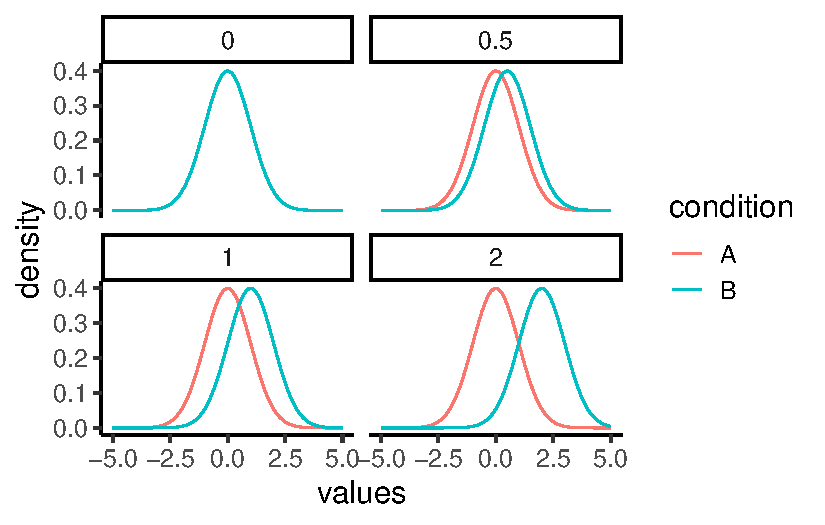
\includegraphics[width=1\textwidth,height=\textheight]{Supplemental_Chapter---Hypothesis-Testing_files/figure-pdf/fig-5.5effectdists-1.pdf}

}

\caption{\label{fig-5.5effectdists}Each panel shows hypothetical
distributions for two conditions. As the effect-size increases, the
difference between the distributions become larger.}

\end{figure}

The remaining panels are hypothetical examples of what a true effect
could look like, when your manipulation actually causes a difference.
For example, if condition A is a control group, and condition B is a
treatment group, we are looking at three cases where the treatment
manipulation causes a positive shift in the mean of distribution. We are
using normal curves with mean =0 and sd =1 for this demonstration, so a
shift of .5 is a shift of half of a standard deviation. A shift of 1 is
a shift of 1 standard deviation, and a shift of 2 is a shift of 2
standard deviations. We could draw many more examples showing even
bigger shifts, or shifts that go in the other direction.

Let's look at another example, but this time we'll use some concrete
measurements. Let's say we are looking at final exam performance, so our
numbers are grade percentages. Let's also say that we know the mean on
the test is 65\%, with a standard deviation of 5\%. Group A could be a
control that just takes the test, Group B could receive some
``educational'' manipulation designed to improve the test score. These
graphs then show us some hypotheses about what the manipulation may or
may not be doing.

\begin{figure}

{\centering 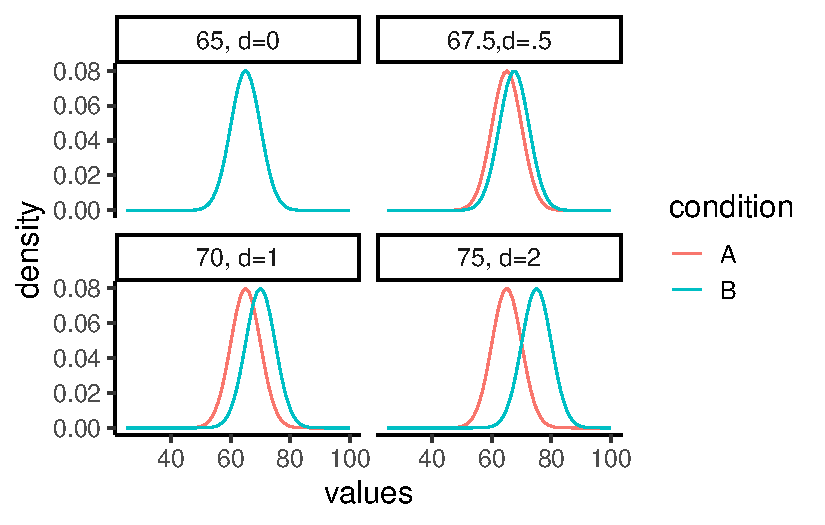
\includegraphics[width=1\textwidth,height=\textheight]{Supplemental_Chapter---Hypothesis-Testing_files/figure-pdf/fig-5.5effectdistsB-1.pdf}

}

\caption{\label{fig-5.5effectdistsB}Each panel shows hypothetical
distributions for two conditions. As the effect-size increases, the
difference between the distributions become larger.}

\end{figure}

The first panel shows that both condition A and B will sample test
scores from the same distribution (mean =65, with 0 effect). The other
panels show shifted mean for condition B (the treatment that is supposed
to increase test performance). So, the treatment could increase the test
performance by 2.5\% (mean 67.5, .5 sd shift), or by 5\% (mean 70, 1 sd
shift), or by 10\% (mean 75\%, 2 sd shift), or by any other amount. In
terms of our previous metaphor, a shift of 2 standard deviations is more
like jack-hammer in terms of size, and a shift of .5 standard deviations
is more like using a pencil. The thing about research, is we often have
no clue about whether our manipulation will produce a big or small
effect, that's why we are conducting the research.

You might have noticed that the letter \(d\) appears in the above
figure. Why is that? Jacob Cohen {[}@cohen1988{]} used the letter \(d\)
in defining the effect-size for this situation, and now everyone calls
it Cohen's \(d\). The formula for Cohen's \(d\) is:

\(d = \frac{\text{mean for condition 1} - \text{mean for condition 2}}{\text{population standard deviation}}\)

If you notice, this is just a kind of z-score. It is a way to
standardize the mean difference in terms of the population standard
deviation.

It is also worth noting again that this measure of effect-size is
entirely hypothetical for most purposes. In general, researchers do not
know the population standard deviation, they can only guess at it, or
estimate it from the sample. The same goes for means, in the formula
these are hypothetical mean differences in two population distributions.
In practice, researchers do not know these values, they guess at them
from their samples.

Before discussing why the concept of effect-size can be useful, we note
that Cohen's \(d\) is useful for understanding abstract measures. For
example, when you don't know what a difference of 10 or 20 means as a
raw score, you can standardize the difference by the sample standard
deviation, then you know roughly how big the effect is in terms of
standard units. If you thought a 20 was big, but it turned out to be
only 1/10th of a standard deviation, then you would know the effect is
actually quite small with respect to the overall variability in the
data.

\hypertarget{power}{%
\subsection{Power}\label{power}}

When there is a true effect out there to measure, you want to make sure
your design is sensitive enough to detect the effect, otherwise what's
the point. We've already talked about the idea that an effect can have
different sizes. The next idea is that your design can be more less
sensitive in its ability to reliabily measure the effect. We have
discussed this general idea many times already in the textbook, for
example we know that we will be more likely to detect ``significant''
effects (when there are real differences) when we increase our
sample-size. Here, we will talk about the idea of design sensitivity in
terms of the concept of power. Interestingly, the concept of power is a
somewhat limited concept, in that it only exists as a concept within
some philosophies of statistics.

\hypertarget{a-digresssion-about-hypothesis-testing}{%
\subsubsection{A digresssion about hypothesis
testing}\label{a-digresssion-about-hypothesis-testing}}

In particular, the concept of power falls out of the Neyman-Pearson
concept of null vs.~alternative hypothesis testing. Up to this point, we
have largely avoided this terminology. This is perhaps a disservice in
that the Neyman-Pearson ideas are by now the most common and widespread,
and in the opinion of some of us, they are also the most widely
misunderstood and abused idea, which is why we have avoided these ideas
until now.

What we have been mainly doing is talking about hypothesis testing from
the Fisherian (Sir Ronald Fisher, the ANOVA guy) perspective. This is a
basic perspective that we think can't be easily ignored. It is also
quite limited. The basic idea is this:

\begin{enumerate}
\def\labelenumi{\arabic{enumi}.}
\tightlist
\item
  We know that chance can cause some differences when we measure
  something between experimental conditions.
\item
  We want to rule out the possibility that the difference that we
  observed can not be due to chance
\item
  We construct large N designs that permit us to do this when a real
  effect is observed, such that we can confidently say that big
  differences that we find are so big (well outside the chance window)
  that it is highly implausible that chance alone could have produced.
\item
  The final conclusion is that chance was extremely unlikely to have
  produced the differences. We then infer that something else, like the
  manipulation, must have caused the difference.
\item
  We don't say anything else about the something else.
\item
  We either reject the null distribution as an explanation (that chance
  couldn't have done it), or retain the null (admit that chance could
  have done it, and if it did we couldn't tell the difference between
  what we found and what chance could do)
\end{enumerate}

Neyman and Pearson introduced one more idea to this mix, the idea of an
alternative hypothesis. The alternative hypothesis is the idea that if
there is a true effect, then the data sampled into each condition of the
experiment must have come from two different distributions. Remember,
when there is no effect we assume all of the data cam from the same
distribution (which by definition can't produce true differences in the
long run, because all of the numbers are coming from the same
distribution). The graphs of effect-sizes from before show examples of
these alternative distributions, with samples for condition A coming
from one distribution, and samples from condition B coming from a
shifted distribution with a different mean.

So, under the Neyman-Pearson tradition, when a researcher find a
signifcant effect they do more than one things. First, they reject the
null-hypothesis of no differences, and they accept the alternative
hypothesis that there was differences. This seems like a sensible thing
to do. And, because the researcher is actually interested in the
properties of the real effect, they might be interested in learning more
about the actual alternative hypothesis, that is they might want to know
if their data come from two different distributions that were separated
by some amount\ldots in other words, they would want to know the size of
the effect that they were measuring.

\hypertarget{back-to-power}{%
\subsubsection{Back to power}\label{back-to-power}}

We have now discussed enough ideas to formalize the concept of
statistical power. For this concept to exist we need to do a couple
things.

\begin{enumerate}
\def\labelenumi{\arabic{enumi}.}
\tightlist
\item
  Agree to set an alpha criterion. When the p-value for our
  test-statistic is below this value we will call our finding
  statistically significant, and agree to reject the null hypothesis and
  accept the ``alternative'' hypothesis (sidenote, usually it isn't very
  clear which specific alternative hypothesis was accepted)
\item
  In advance of conducting the study, figure out what kinds of
  effect-sizes our design is capable of detecting with particular
  probabilites.
\end{enumerate}

The power of a study is determined by the relationship between

\begin{enumerate}
\def\labelenumi{\arabic{enumi}.}
\tightlist
\item
  The sample-size of the study
\item
  The effect-size of the manipulation
\item
  The alpha value set by the researcher.
\end{enumerate}

To see this in practice let's do a simulation. We will do a t-test on a
between-groups design 10 subjects in each group. Group A will be a
control group with scores sampled from a normal distribution with mean
of 10, and standard deviation of 5. Group B will be a treatment group,
we will say the treatment has an effect-size of Cohen's \(d\) = .5,
that's a standard deviation shift of .5, so the scores with come from a
normal distribution with mean =12.5 and standard deivation of 5.
Remember 1 standard deviation here is 5, so half of a standard deviation
is 2.5.

The following R script runs this simulated experiment 1000 times. We set
the alpha criterion to .05, this means we will reject the null whenever
the \(p\)-value is less than .05. With this specific design, how many
times out of of 1000 do we reject the null, and accept the alternative
hypothesis?

\begin{verbatim}
#> [1] 180
\end{verbatim}

The answer is that we reject the null, and accept the alternative 180
times out of 1000. In other words our experiment succesfully accepts the
alternative hypothesis 18 percent of the time, this is known as the
power of the study. Power is the probability that a design will
succesfully detect an effect of a specific size.

Importantly, power is completely abstract idea that is completely
determined by many assumptions including N, effect-size, and alpha. As a
result, it is best not to think of power as a single number, but instead
as a family of numbers.

For example, power is different when we change N. If we increase N, our
samples will more precisely estimate the true distributions that they
came from. Increasing N reduces sampling error, and shrinks the range of
differences that can be produced by chance. Lets' increase our N in this
simulation from 10 to 20 in each group and see what happens.

\begin{verbatim}
#> [1] 334
\end{verbatim}

Now the number of significant experiments i 334 out of 1000, or a power
of 33.4 percent. That's roughly doubled from before. We have made the
design more sensitive to the effect by increasing N.

We can change the power of the design by changing the alpha-value, which
tells us how much evidence we need to reject the null. For example, if
we set the alpha criterion to 0.01, then we will be more conservative,
only rejecting the null when chance can produce the observed difference
1\% of the time. In our example, this will have the effect of reducing
power. Let's keep N at 20, but reduce the alpha to 0.01 and see what
happens:

\begin{verbatim}
#> [1] 134
\end{verbatim}

Now only 134 out of 1000 experiments are significant, that's 13.4 power.

Finally, the power of the design depends on the actual size of the
effect caused by the manipulation. In our example, we hypothesized that
the effect caused a shift of .5 standard deviations. What if the effect
causes a bigger shift? Say, a shift of 2 standard deviations. Let's keep
N= 20, and alpha \textless{} .01, but change the effect-size to two
standard deviations. When the effect in the real-world is bigger, it
should be easier to measure, so our power will increase.

\begin{verbatim}
#> [1] 1000
\end{verbatim}

Neat, if the effect-size is actually huge (2 standard deviation shift),
then we have power 100 percent to detect the true effect.

\hypertarget{power-curves}{%
\subsubsection{Power curves}\label{power-curves}}

We mentioned that it is best to think of power as a family of numbers,
rather than as a single number. To elaborate on this consider the power
curve below. This is the power curve for a specific design: a between
groups experiments with two levels, that uses an independent samples
t-test to test whether an observed difference is due to chance.
Critically, N is set to 10 in each group, and alpha is set to .05

In Figure~\ref{fig-5.5powercurve} power (as a proportion, not a
percentage) is plotted on the y-axis, and effect-size (Cohen's d) in
standard deviation units is plotted on the x-axis.

\begin{figure}

{\centering 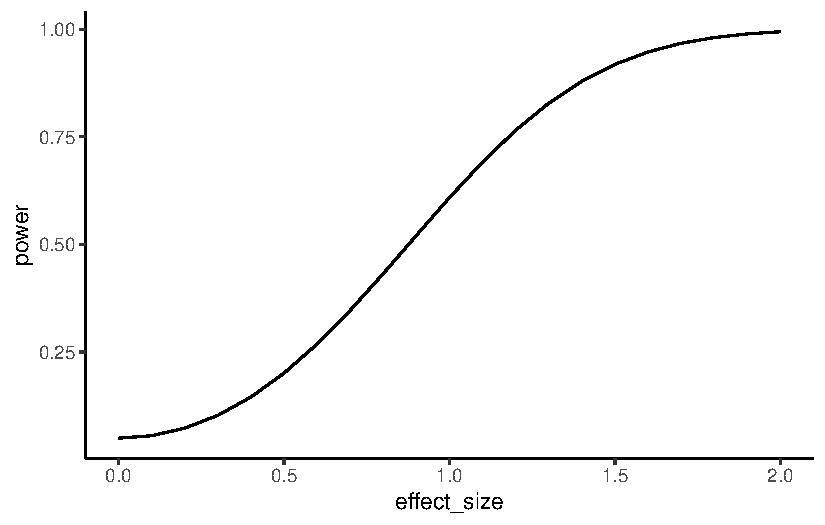
\includegraphics[width=1\textwidth,height=\textheight]{Supplemental_Chapter---Hypothesis-Testing_files/figure-pdf/fig-5.5powercurve-1.pdf}

}

\caption{\label{fig-5.5powercurve}This figure shows power as a function
of effect-size (Cohen's d) for a between-subjects independent samples
t-test, with N=10, and alpha criterion 0.05.}

\end{figure}

A power curve like this one is very helpful to understand the
sensitivity of a particular design. For example, we can see that a
between subjects design with N=10 in both groups, will detect an effect
of d=.5 (half a standard deviation shift) about 20\% of the time, will
detect an effect of d=.8 about 50\% of the time, and will detect an
effect of d=2 about 100\% of the time. All of the percentages reflect
the power of the design, which is the percentage of times the design
would be expected to find a \(p\) \textless{} 0.05.

Let's imagine that based on prior research, the effect you are
interested in measuring is fairly small, d=0.2. If you want to run an
experiment that will detect an effect of this size a large percentage of
the time, how many subjects do you need to have in each group? We know
from the above graph that with N=10, power is very low to detect an
effect of d=0.2. Let's make Figure~\ref{fig-5.5powercurveN} and vary the
number of subjects rather than the size of the effect.

\begin{figure}

{\centering 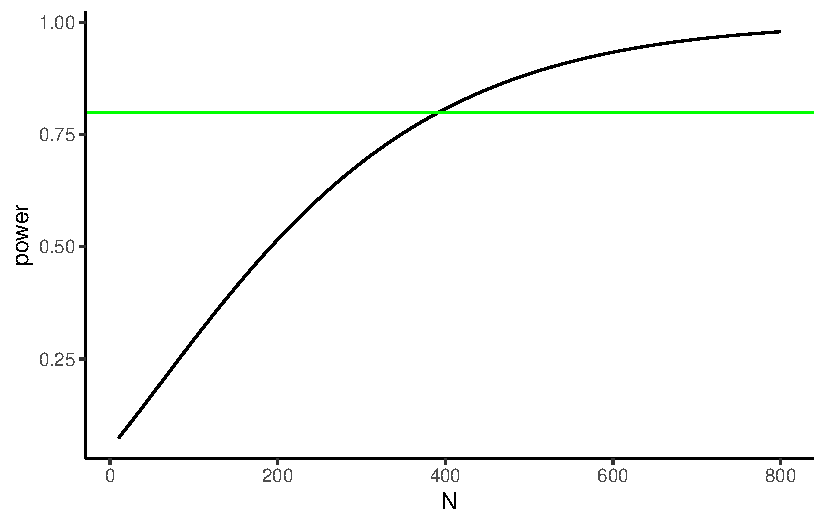
\includegraphics[width=1\textwidth,height=\textheight]{Supplemental_Chapter---Hypothesis-Testing_files/figure-pdf/fig-5.5powercurveN-1.pdf}

}

\caption{\label{fig-5.5powercurveN}This figure shows power as a function
of N for a between-subjects independent samples t-test, with d=0.2, and
alpha criterion 0.05.}

\end{figure}

The figure plots power to detect an effect of d=0.2, as a function of N.
The green line shows where power = .8, or 80\%. It looks like we would
nee about 380 subjects in each group to measure an effect of d=0.2, with
power = .8. This means that 80\% of our experiments would succesfully
show p \textless{} 0.05. Often times power of 80\% is recommended as a
reasonable level of power, however even when your design has power =
80\%, your experiment will still fail to find an effect (associated with
that level of power) 20\% of the time!

\hypertarget{planning-your-design}{%
\subsection{Planning your design}\label{planning-your-design}}

Our discussion of effect size and power highlight the importance of the
understanding the statistical limitations of an experimental design. In
particular, we have seen the relationship between:

\begin{enumerate}
\def\labelenumi{\arabic{enumi}.}
\tightlist
\item
  Sample-size
\item
  Effect-size
\item
  Alpha criterion
\item
  Power
\end{enumerate}

As a general rule of thumb, small N designs can only reliably detect
very large effects, whereas large N designs can reliably detect much
smaller effects. As a researcher, it is your responsibility to plan your
design accordingly so that it is capable of reliably detecting the kinds
of effects it is intended to measure.

\hypertarget{some-considerations}{%
\subsection{Some considerations}\label{some-considerations}}

\hypertarget{low-powered-studies}{%
\subsubsection{Low powered studies}\label{low-powered-studies}}

Consider the following case. A researcher runs a study to detect an
effect of interest. There is good reason, from prior research, to
believe the effect-size is d=0.5. The researcher uses a design that has
30\% power to detect the effect. They run the experiment and find a
significant p-value, (p\textless.05). They conclude their manipulation
worked, because it was unlikely that their result could have been caused
by chance. How would you interpret the results of a study like this?
Would you agree with thte researchers that the manipulation likely
caused the difference? Would you be skeptical of the result?

The situation above requires thinking about two kinds of probabilities.
On the one hand we know that the result observed by the researchers does
not occur often by chance (p is less than 0.05). At the same time, we
know that the design was underpowered, it only detects results of the
expected size 30\% of the time. We are face with wondering what kind of
luck was driving the difference. The researchers could have gotten
unlucky, and the difference really could be due to chance. In this case,
they would be making a type I error (saying the result is real when it
isn't). If the result was not due to chance, then they would also be
lucky, as their design only detects this effect 30\% of the time.

Perhaps another way to look at this situation is in terms of the
replicability of the result. Replicability refers to whether or not the
findings of the study would be the same if the experiment was repeated.
Because we know that power is low here (only 30\%), we would expect that
most replications of this experiment would not find a significant
effect. Instead, the experiment would be expected to replicate only 30\%
of the time.

\hypertarget{large-n-and-small-effects}{%
\subsubsection{Large N and small
effects}\label{large-n-and-small-effects}}

Perhaps you have noticed that there is an intriguiing relationship
between N (sample-size) and power and effect-size. As N increases, so
does power to detect an effect of a particular size. Additionally, as N
increases, a design is capable of detecting smaller and smaller effects
with greater and greater power. For example, if N was large enough, we
would have high power to detect very small effects, say d= 0.01, or even
d=0.001. Let's think about what this means.

Imagine a drug company told you that they ran an experiment with 1
billion people to test whether their drug causes a significant change in
headache pain. Let's say they found a significant effect (with power
=100\%), but the effect was very small, it turns out the drug reduces
headache pain by less than 1\%, let's say 0.01\%. For our imaginary
study we will also assume that this effect is very real, and not caused
by chance.

Clearly the design had enough power to detect the effect, and the effect
was there, so the design did detect the effect. However, the issue is
that there is little practical value to this effect. Nobody is going to
by a drug to reduce their headache pain by 0.01\%, even if it was
``scientifcally proven'' to work. This example brings up two issues.
First, increasing N to very large levels will allow designs to detect
almost any effect (even very tiny ones) with very high power. Second,
sometimes effects are meaningless when they are very small, especially
in applied research such as drug studies.

These two issues can lead to interesting suggestions. For example,
someone might claim that large N studies aren't very useful, because
they can always detect really tiny effects that are practically
meaningless. On the other hand, large N studies will also detect larger
effects too, and they will give a better estimate of the ``true'' effect
in the population (because we know that larger samples do a better job
of estimating population parameters). Additionally, although really
small effects are often not interesting in the context of applied
research, they can be very important in theoretical research. For
example, one theory might predict that manipulating X should have no
effect, but another theory might predict that X does have an effect,
even if it is a small one. So, detecting a small effect can have
theoretical implication that can help rule out false theories. Generally
speaking, researchers asking both theoretical and applied questions
should think about and establish guidelines for ``meaningful''
effect-sizes so that they can run designs of appropriate size to detect
effects of ``meaningful size''.

\hypertarget{small-n-and-large-effects}{%
\subsubsection{Small N and Large
effects}\label{small-n-and-large-effects}}

All other things being equal would you trust the results from a study
with small N or large N? This isn't a trick question, but sometimes
people tie themselves into a knot trying to answer it. We already know
that large sample-sizes provide better estimates of the distributions
the samples come from. As a result, we can safely conclude that we
should trust the data from large N studies more than small N studies.

At the same time, you might try to convince yourself otherwise. For
example, you know that large N studies can detect very small effects
that are practically and possibly even theoretically meaningless. You
also know that that small N studies are only capable of reliably
detecting very large effects. So, you might reason that a small N study
is better than a large N study because if a small N study detects an
effect, that effect must be big and meaningful; whereas, a large N study
could easily detect an effect that is tiny and meaningless.

This line of thinking needs some improvement. First, just because a
large N study can detect small effects, doesn't mean that it only
detects small effects. If the effect is large, a large N study will
easily detect it. Large N studies have the power to detect a much wider
range of effects, from small to large. Second, just because a small N
study detected an effect, does not mean that the effect is real, or that
the effect is large. For example, small N studies have more variability,
so the estimate of the effect size will have more error. Also, there is
5\% (or alpha rate) chance that the effect was spurious. Interestingly,
there is a pernicious relationship between effect-size and type I error
rate

\hypertarget{type-i-errors-are-convincing-when-n-is-small}{%
\subsubsection{Type I errors are convincing when N is
small}\label{type-i-errors-are-convincing-when-n-is-small}}

So what is this pernicious relationship between Type I errors and
effect-size? Mainly, this relationship is pernicious for small N
studies. For example, the following figure illustrates the results of
1000s of simulated experiments, all assuming the null distribution. In
other words, for all of these simulations there is no true effect, as
the numbers are all sampled from an identical distribution (normal
distribution with mean =0, and standard deviation =1). The true
effect-size is 0 in all cases.

We know that under the null, researchers will find p values that are
less 5\% about 5\% of the time, remember that is the definition. So, if
a researcher happened to be in this situation (where there manipulation
did absolutely nothing), they would make a type I error 5\% of the time,
or if they conducted 100 experiments, they would expect to find a
significant result for 5 of them.

Figure~\ref{fig-5.5effectsizeType1} reports the findings from only the
type I errors, where the simulated study did produce p \textless{} 0.05.
For each type I error, we calculated the exact p-value, as well as the
effect-size (cohen's D) (mean difference divided by standard deviation).
We already know that the true effect-size is zero, however take a look
at this graph, and pay close attention to the smaller sample-sizes.

\begin{figure}

{\centering 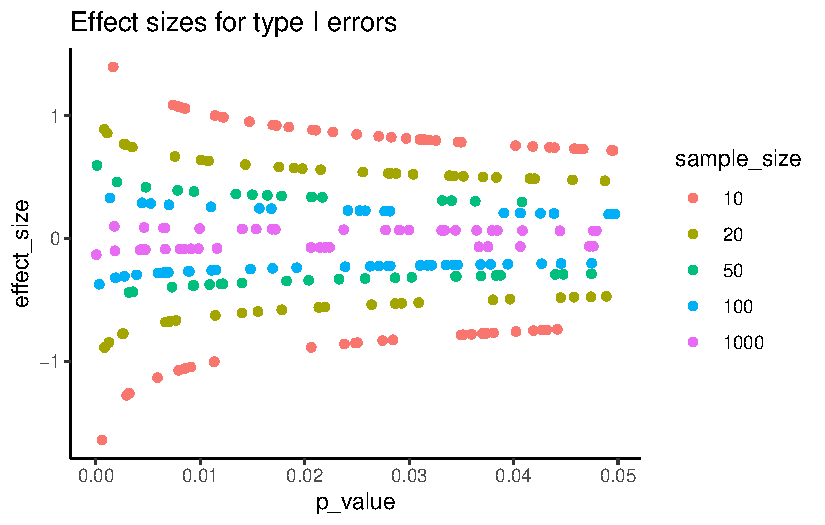
\includegraphics[width=1\textwidth,height=\textheight]{Supplemental_Chapter---Hypothesis-Testing_files/figure-pdf/fig-5.5effectsizeType1-1.pdf}

}

\caption{\label{fig-5.5effectsizeType1}Effect size as a function of
p-values for type 1 Errors under the null, for a paired samples t-test.}

\end{figure}

For example, look at the red dots, when sample size is 10. Here we see
that the effect-sizes are quite large. When p is near 0.05 the
effect-size is around .8, and it goes up and up as when p gets smaller
and smaller. What does this mean? It means that when you get unlucky
with a small N design, and your manipulation does not work, but you by
chance find a ``significant'' effect, the effect-size measurement will
show you a ``big effect''. This is the pernicious aspect. When you make
a type I error for small N, your data will make you think there is no
way it could be a type I error because the effect is just so big!.
Notice that when N is very large, like 1000, the measure of effect-size
approaches 0 (which is the true effect-size in the simulation shown in
Figure~\ref{fig-5.5cohensD}).

\begin{figure}

{\centering 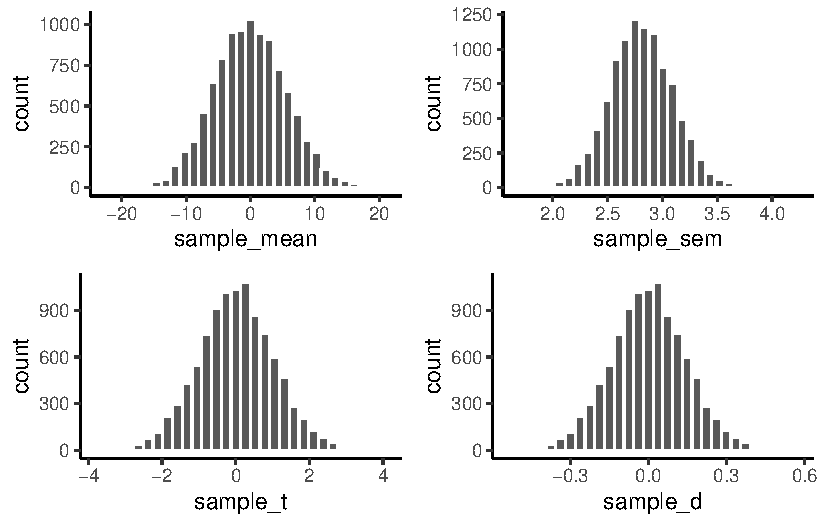
\includegraphics[width=1\textwidth,height=\textheight]{Supplemental_Chapter---Hypothesis-Testing_files/figure-pdf/fig-5.5cohensD-1.pdf}

}

\caption{\label{fig-5.5cohensD}Each panel shows a histogram of a
different sampling statistic.}

\end{figure}



\end{document}
